\documentclass{article}
\usepackage[latin1]{inputenc}
\usepackage[pdftex]{color}
\usepackage[pdftex]{graphicx}
\usepackage[T1]{fontenc}
\usepackage{amsfonts}
\usepackage{amsmath}
\usepackage{cancel}
\usepackage{array}
\usepackage{xspace}
\usepackage{verbatim}
\usepackage{mathabx}
\usepackage{longtable}
\setlength{\parindent}{0pt}
\usepackage{url}
\usepackage{hyperref}

\title{GenAMap Data Importing}
\author{}
\date{}

\begin{document}

\maketitle
\tableofcontents
\vspace{1cm}

For further questions / comments / suggestions, please contact \url{genamapsupport@cs.cmu.edu}.

\section{Introduction}

In this tutorial, we describe how data should be formatted for importing into GenAMap. Data formatting is one of the trickier aspects of GenAMap. As it is impossible, from a development standpoint, to cater to all possible formats in which data may be available to the user, he or she will often have to go through a data pre-processing step. \\

The format of choice in GenAMap is the delimited text-file. We chose this format because it can be easily generated from a wide variety of applications (e.g. Microsoft Excel, SQL, Matlab, etc.). For example, if the data is given as a spreadsheet, the user can click ``save as'' and choose a comma-delimited or tab-delimited text format for saving the data from within Microsoft Excel or other Office applications. \\

Before importing data, GenAMap parses and checks any data file to ensure it is formatted correctly. Hence, it is unlikely that bogus data is erroneously imported. However, it is still advisable that the user reads the instructions in this document carefully if they wish to import a data set of a certain type. \\

GenAMap comes with an example data set for every available data format. These can be found in the `Documentation/ExampleData' folder. Also, you can find video walkthroughs on the GenAMap website that demonstrate how to bring up and fill out the importing dialogs. These can be found under \url{http://sailing.cs.cmu.edu/genamap/tutorials.html}.

\section{Importing Marker Data}

\paragraph{Overview} Marker Data has three components: The actual marker (=SNP) values, labels for each sample / individual, and labels for each marker. The marker values take the form of an $N$ by $d$ matrix where $N$ is the number of samples and $d$ is the number of markers. Each row corresponds to a sample, each column corresponds to a marker and each entry represents the value of the marker corresponding to the column of the entry for the sample corresponding to the row of the entry. A sample label is a simple string. A marker label has three components: A marker name, the number of the chromosome the marker is on and the location of the marker along that chromosome (in base pairs).

\paragraph{How to format the data} Please provide the data as three files: a marker value file, a sample label file and a marker label file. The sample label file is optional. The marker value file should be an $N$ by $d$ matrix (as described above) in a delimited format, where the delimiter may be a tab, a space or a comma. It should only contain numerical values. The sample labels should be in a file with $N$ lines, where each line is the label for a particular sample. These can be arbitrary but have to be unique and at most 30 characters long. If the sample label file is not provided, GenAMap assigns sample labels `S1', `S2', `S3', .. etc. The marker labels should be arranged as a $d$ by 3 tab-delimited matrix, where each line contains the the marker name, the number of the chromosome the marker is on and the marker location in base pairs, in that order from left to right. It is possible to omit chromosome number and marker location. In that case, the marker label file simply has $d$ lines, where each line contains the marker name, and GenAMap will fill in dummy values for chromosome number and marker location. The marker names can be arbitrary (at most 30 characters) and the chromosome number and marker location must be positive integers, and no pair of (chromosome number, marker location) may appear twice. Also, no marker name may appear twice. While the values of $N$ and $d$ that define the sizes of these files can be arbitrary, they have to be consistent across the three files.\\

Marker Data can be used to run association algorithms and other algorithms. Note that while it is permitted for marker values to take any numerical form, including floating-point values, a few algorithms (currently PLINK, Structure and Population Analysis) incorporated in GenAMap do not work unless the marker value matrix only contains values 0,1 and 2. (These values should indicate the number of minor alleles of the sample at the respective marker location.) The chromosome number and marker location are used in the chromosome browser and to the define the x-axis in the Manhattan plot. The marker name is used to link to dbSNP and SGD (Saccharomyces Genome Database). In order to interact successfully with these external databases through GenAMap, the marker name must be an rs\# (for dbSNP) or the name of the gene the marker is on (for SGD). The sample labels have no special purpose except to co-interpret different data sets that pertain to the same samples.

\paragraph{How to import the data} 
\begin{enumerate}
\item Bring up the marker import dialog
\item Choose the project to add the data to
\item Choose the name of the Marker Data set itself
\item Provide the paths to the input files
\item Choose the applicable delimiter
\item Check the `import w/o chromosome location' box if this information is not specified in the marker label file
\item Check `import w/o data' if you only want to import marker labels, but no marker values
\item Click `Import'
\end{enumerate}

Figure \ref{marker} shows two ways to fill out the marker import dialog using the data in the ExampleData folder.

\paragraph{Video Tutorial} For a visual demonstration of the importing process, please view the `Importing markers tutorial' video on the GenAMap website.

\paragraph{Example data files} We provide 5 files: markerVals.txt, markerLabels.txt, markerLabelsReal.txt, markerLabelsDummy.txt and sampleLabels.txt. These can be used directly for importing. markerLabelsReal.txt contains examples of actual markers with name and location. You can use these marker names to access he SGD database. Note that the actual marker values (as well as all other numerical data) provided for the purposes of this tutorial are synthetic and any resemblance to real data is coincidental. markerLabels.txt omits chromosome number and marker location and hence has only a single columns. markerLabelsDummy.txt contains dummy locations. In fact, using markerLabels.txt and using markerLabelsDummy.txt has identical results as GenAMap would fill in exactly these dummy locations to complete the dataset. sampleLabels.txt contains exactly the sample labels that GenAMap would provide if the sample label file is omitted during importing.

\section{Importing Trait Data}

\paragraph{Overview} Trait data in GenAMap can stand for gene expression data or phenotype data. Similar to Marker Data, Trait Data has three components: The actual trait values, labels for each sample / individual and labels for each trait. The trait values take the form of an $N$ by $t$ matrix where $N$ is the number of samples and $t$ is the number of traits. Each row corresponds to a sample, each column corresponds to a trait and each entry represents the value of the trait corresponding to the column of the entry for the sample corresponding to the row of the entry. Sample labels and trait labels are both simple strings.

\paragraph{How to format the data} There are different options for providing this data. Either, we use three files - one for the trait values, one for the sample labels and one of the trait labels - as we did for marker data, or we provide all this information in a single file. \\

In the case of separate files, the trait value file should be either a delimited $N$ by $t$ matrix (as described above) or a delimited $t$ by $N$ matrix which would correspond to the transpose of the aforementioned matrix. In any case, this file should only contain numerical entries. Acceptable delimiters are tabs, whitespaces or commas. This file should only contain numerical values. The sample labels and trait labels should each be in a file with $N$ / $t$ lines respectively, where each line is the label for a particular sample / trait. These can be arbitrary but no label may appear twice in the same file and they may not exceed 30 characters. As for markers, the sample label file is optional. If it is not provided, the system generates dummy sample labels as such: `S1', `S2', `S3', .. While the numbers $N$ and $t$ that determine the size of these files are arbitrary, they must be consistent across the three files.\\

In the case all information is contained in a single file, the file should take the form of either an $N+1$ by $t+1$ delimited matrix or a $t+1$ by $N+1$ delimited matrix where the first row / column contains the sample labels / trait labels as headers. All entries except the first row / column should be numerical. The first entry in the first row should be empty.\\

Trait Data can be used to run association algorithms, network algorithms, and other algorithms. Trait labels are used to link to external resources Google and UniProt, with the latter only applicable if traits are gene expressions. To use these facilities, trait labels must be interpretable by the external databases. For gene expression traits, trait labels are also used to perform GO analyses. For this, trait labels must take the form of gene names. To see which gene naming conventions GenAMap supports for a particular species, navigate to the folder `goSpecies' and open the file for the species you are interested in. The trait labels should appear in this table to facilitate GO analysis. If different Trait Data sets / Marker Data sets are to be used within the same algorithm, the sample label files provided for them must contain the same samples. They are then used to determine which marker values / trait values correspond to the same sample.

\paragraph{How to import the data} 
\begin{enumerate}
\item Bring up the trait import dialog
\item Choose the project to add the data to
\item Choose the name of the Trait Data set itself
\item Provide the paths to the input files. Only use the `Trait File' if labels are specified as headers.
\item Choose the species that your data pertains to. This information is used to facilitate GO analysis if the trait labels are valid gene names.
\item If you provided trait labels (and possibly sample labels) as separate files, choose the radio button `no row or columns headers'. If labels are contained as headers in the `Trait file', choose the radio button `row \& column headers'.
\item Choose between the radio buttons `Nxt' and `txN' depending on the orientation of your trait matrix
\item Choose the correct delimiter
\item To import only labels without data, tick `import w/o data'
\end{enumerate}

Figure \ref{trait} shows two ways to fill out the trait import dialog using the data in the ExampleData folder.

\paragraph{Video Tutorial}

For a visual demonstration of the importing process, please view the `Importing traits tutorial' video on the GenAMap website.

\paragraph{Example data files} We provide 8 files: geneVals.txt, geneLabels.txt, traitValsNxt.txt, traitValstxN.txt, traitValsNxtwithHeaders.txt, traitValstxNwithHeaders.txt, traitLabels.txt and sampleLabels.txt. These can be used directly for importing. geneVals.txt, geneLabels.txt and sampleLabels.txt go together. These represent a synthetic gene expression data set. The labels used in geneLabels.txt are gene names from yeast, so during import we select the species `Saccharomyces cerevisiae' (see the top part of Figure \ref{trait}). The four files whose name starts with `traitVals' all contain the same data, either transposed or not transposed, and either with or without headers. traitValsNxt.txt and traitValstxN.txt contain no headers and can be used with sampleLabels.txt and traitLabels.txt. The trait labels used here are dummy labels. Hence, we do not select a species during import (see the bottom part of Figure \ref{trait}).

\section{Importing other data}

\subsection{Network Data}

Networks are edge-weight matrices of graphs over traits. Hence, they take the form of a square, symmetric, real-valued matrix. They can only be imported referencing an already existing Trait Data set. The data can be provided in one of two ways: As a tab-delimited matrix of size $t$ by $t$, where $t$ is the number of traits in the referenced Trait Data set, or as an $e$ by 3 tab-delimited matrix where each row corresponds to a single edge in the Network. \\

In the tab-delimited format, each row / column corresponds to a trait in the Trait Data set that the Network references. In that Trait Data set, the traits are in a certain order as specified by the trait labels that were used when importing that data set. That ordering must be the same as the ordering of the traits in the $t$ by $t$ network matrix, even though the labels are omitted. The matrix contained in the file must be symmetric.\\

If providing the data in an edgewise format, each row must contain three entries: The first two entries should be the labels of the traits that the edge connects (these labels were given when importing the Trait Data set) and the third entry should be the weight of the edge. Please note that no edge may appear more than once in the file. So, for example, if one entry is `T1 T2 0.43', then having another entry `T2 T1 0.43' is illegal.\\

To import the data, bring up the network dialog as in Figure \ref{network}. Choose the project to add the data to, the Trait Data set the Network is for, and the name of the Network itself. Click the radio buttons `Load from File' and choose your file format (`Tab delimited' or `Edge by edge'), provide the path to the file and click `Run'. The example files are `traitNetworkDelimFormat.txt', `traitNetworkEdgeFormat.txt' and `geneNetwork.txt'. These contain the ground truth networks for the provided Trait Data sets. The relevant video is `Adding network structure tutorial'.

\subsection{Association Data}

Association Data sets describe the association strengths between markers and traits. They can only be imported referencing an already existing Marker Data set and an already existing Trait Data set. The association file should take the form of a $d$ by $t$ matrix, where $d$ is the number of markers in the referenced Marker Data set and $t$ is the number of traits in the referenced Trait Data set. The $i,j$'th entry is the association strength between marker $i$ and trait $j$. The data should be provided as a tab-delimited matrix with numerical entries. The order of the rows / columns in the association file should match the order of the marker labels / trait labels that were provided when the referenced Marker Data set / Trait Data set was imported.\\

To import the data, bring up the import dialog as in Figure \ref{association}. Choose the project to add the data to, the name of the Marker Data set and Trait Data sets the Association Data set is for, and the name of the Association Data set itself. Click the radio button `Load from File', provide the path to the file and click `Run'. The example files are `traitAssociations.txt' and `geneAssociations.txt'. These are the ground truth associations between the provided Marker Data set and the two provided Trait Data sets. The relevant video is `Running association algorithms tutorial'.

\subsection{Clustering}

A Clustering is a re-ordering / permutation of traits that pulls related traits close together. It always references a Trait Data set. This data should be imported as a single file with $t$ rows, where $t$ is the number of traits in the referenced Trait Data set. Each row is an integer between 1 and $t$ and corresponds to the index of a trait. These indexes are defined by the ordering of the traits in the Trait Data set. Each index must appear exactly once.\\

To import the data, bring up the import dialog as in Figure \ref{clustering}. Choose the project to add the data to, the name of the Trait Data set the Clustering is for, and the name of the Clustering itself. Click the radio button `Load from File', provide the path to the file and click `Run'. The example file is `traitClustering.txt'. It is the ``ground truth Clustering'' for `traitVals.txt'. If you import `traitNetwork.txt' and `traitClustering.txt' and apply the latter to the former in the Matrix View, the structure in the data will be exposed. The data type `Clustering' is closely tied to the Matrix View in GenAMap. Helpful information can be found in the video `How to use GenAMap's matrix view tutorial'.

\subsection{Subset}

A Subset is a list of traits from a Trait Data set that can be used to direct GenAMap's visualization tools to places of interest, for example by enabling the user to view all traits with a certain used-defined property in a JUNG view. It always references a Trait Data set. Each line in the subset file should contain a single trait label, or a single trait index. The subset will then simply be the set of traits with those labels / indexes.\\

To import the data, bring up the import dialog as in Figure \ref{subset}. Choose the project to add the data to, the name of the Trait Data set the Subset is for and the name of the Subset itself. Click the radio button `Load from File' and then either `Name format' (if your file contains labels) or `Index format' (if your file contains indexes), provide the path to the file and click `Make Subset'. The example file is `traitSubset.txt'. It contains the most interesting traits in `traitVals.txt'. The relevant video is `Trait subset overview tutorial'.

\subsection{Feature Data}

Feature Data represents a quantitative property that can be added to all markers in a Marker Data set. Features can, for example, be used to run the Adaptive Multi-Task Lasso. A Feature always references a Maker Data set. The feature file should be a $d+1$ by $f$ tab-delimited matrix, where $d$ is the number of markers in the Marker Data set and $f$ is the number of features imported. (While each feature is added independently to the Marker Data set, it is possible to specify multiple features in the same file.)The first row of the matrix indicates the names of the features in string format. The remaining $d$ rows contain the actual feature values, which can be arbitrary floating-point numbers. Feature names must be unique and may be at most 30 characters long. The rows of the feature file must align with the columns of the marker value file. Specifically, the marker corresponding to the $i$'th column in the marker value file used to create the referenced Marker Data set should be the marker corresponding to the $i+1$'st row in the feature file (remember, the $i+1$'st row is the $i$'th non-header row).\\

To import the data, bring up the import dialog as in Figure \ref{features}. Choose the project to add the data to and the Marker Data to reference. Provide the path to the file and click `import'. The example file is `features.txt'. The relevant video is `Running AMTL and uploading SNP features'.

\subsection{Tree}

A Tree is a tree-structure over traits in a Trait Data set where the direct path between highly related traits tends to be shorter than the direct path between unrelated traits. The traits themselves correspond to the leaf nodes of the tree. A Tree must reference a Trait Data set. The tree file can be provided in two formats: a parent-child format and a parenthesis format. \\

In the parent-child format, each node in the tree has to be given a name. The leaf nodes have the same names as the labels of the traits they represent. The root node of the tree must have name `root'. All other nodes can have arbitrary names. The tree data file is specified as an $e$ by 2 tab-delimited matrix, where $e$ is the number of edges in the tree. Each row corresponds to an edge. The first entry in each row should be the name of the child node (the one closer to the leaves) and the second entry should be the name of the parent node (the one closer to the root). Note that the number of edges in the tree is equal to the number of nodes in the tree minus one, as each node has exactly one parent apart form the root.\\

In the parenthesis format, each non-leaf node is represented as an opening and closing parenthesis that contains a comma-delimited list of its children. These children may themselves be non-leaf nodes which are represented in such a way. This leads to a nested representation. Leafs (which correspond to traits) are represented by their trait labels. Hence, the representation of each node contains only parentheses, commas and trait labels. (This format can only be used if trait labels themselves contain no commas or parens.) The entire tree can be represented by the expression that describes its root node. Hence, the tree file in the parenthesis format contains just a single (long) line that is the parenthesis representation of the root node.\\

To import the data, bring up the import dialog as in Figure \ref{tree}. Choose the project to add the data to, the Trait Data set the Tree is for, and the name of the Tree itself. Click the radio button `Load from File' and the radio button describing the format of your file. Provide the path to the file and click `Run'. The example files are `traitTreeParentChildFormat.txt' and `traitTreeParenthesisFormat.txt'. These contain the same Tree in different formats. The Tree was built to expose structure in 'traitVals.txt'. The relevant video is `Adding tree data to trait data tutorial'.

\subsection{Population Structure}

A Population Structure in GenAMap is a somewhat complicated data type because it consists of two different components. Firstly, it contain one or more clusterings of the samples in a Marker Data set into populations. Secondly, it contains a low-dimensional embedding of the Marker Data set computed via PCA. (A Population Structure references a Marker Data set.) It is only possible for the user to import the first component (but not the second), and only a single clustering at a time. Once the clustering is imported, GenAMap will automatically start an algorithm that performs PCA on the Marker Data set to fill in this missing component of the Population Structure. To specify the clustering, please provide a $d$ by 2 tab-delimited matrix. The first column should contain the sample labels as provided in the sample label file of the Marker Data set. The second column should contain the cluster assignment of the sample specified in the first column, as an integer between 1 and $k$, with $k$ the total number of clusters. A cluster assignment must be specified for each sample and each cluster between 1 and $k$ must have at least one member. Note that if no sample labels were specified when the Marker Data set was imported, GenAMap created dummy sample labels just as in `sampleLabels.txt'. These can be used to generate the population structure file.\\

To import the data, bring up the import dialog as in Figure \ref{popstruct}. Choose the project to add the data to, the Marker Data set the Population Structure is for and the name of the Population Structure itself. Click the radio button `Load from FIle', provide the path to the file and click `Run'. The example file is `populationStructure.txt'. The relevant video is `Adding and viewing population structure tutorial'.

\subsection{Gene-Trait Association Data and Gene Modules}

At the moment, it is not possible to import these instances of these data types. We apologize for any inconvenience. Those features will be available soon.

\clearpage

\begin{figure}
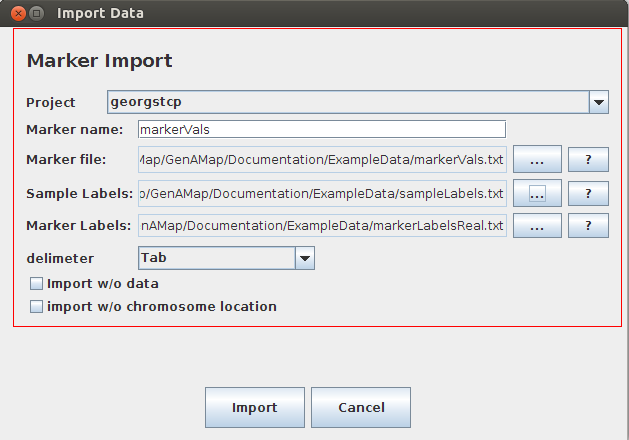
\includegraphics[width=\textwidth]{Figure1a.png}
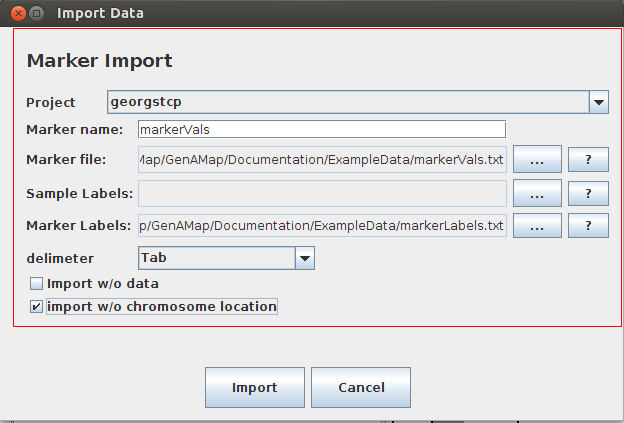
\includegraphics[width=\textwidth]{Figure1b.png}
\caption{\textbf{Importing Marker Data}}
\label{marker}
\end{figure}

\begin{figure}
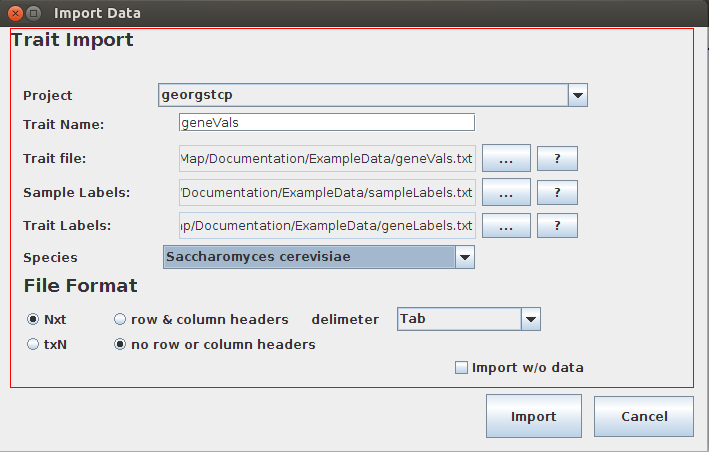
\includegraphics[width=\textwidth]{Figure2a.png}
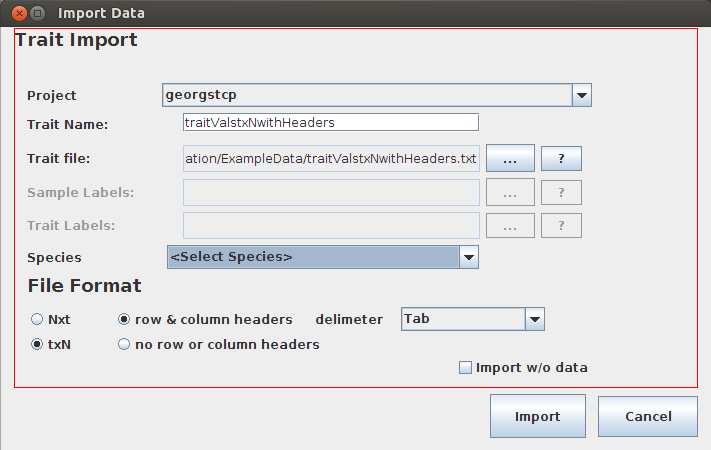
\includegraphics[width=\textwidth]{Figure2b.png}
\caption{\textbf{Importing Trait Data}}
\label{trait}
\end{figure}

\begin{figure}
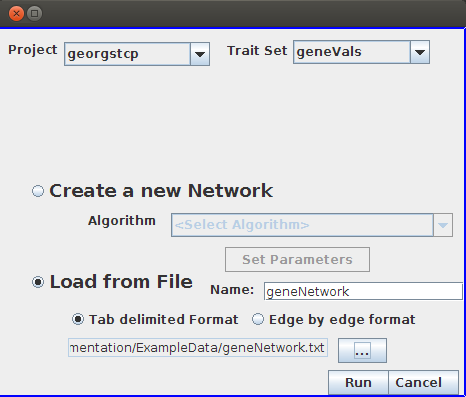
\includegraphics[width=\textwidth]{Figure3.png}
\caption{\textbf{Importing Network Data}}
\label{network}
\end{figure}

\begin{figure}
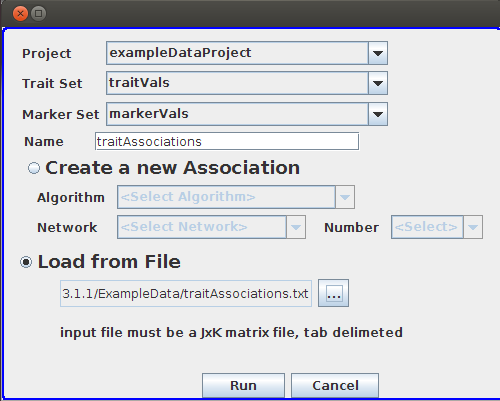
\includegraphics[width=\textwidth]{Figure4.png}
\caption{\textbf{Importing Association Data}}
\label{association}
\end{figure}

\begin{figure}
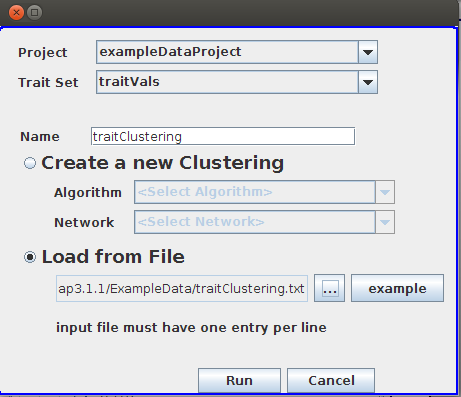
\includegraphics[width=\textwidth]{Figure5.png}
\caption{\textbf{Importing a Clustering}}
\label{clustering}
\end{figure}

\begin{figure}
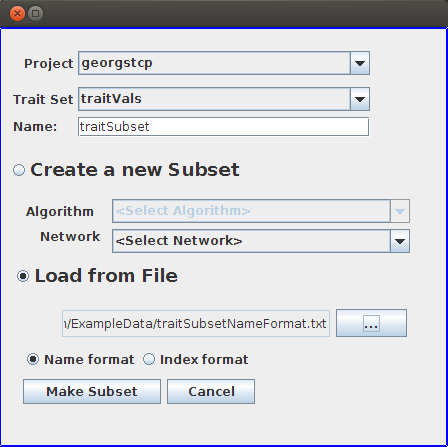
\includegraphics[width=\textwidth]{Figure6.png}
\caption{\textbf{Importing a Subset}}
\label{subset}
\end{figure}

\begin{figure}
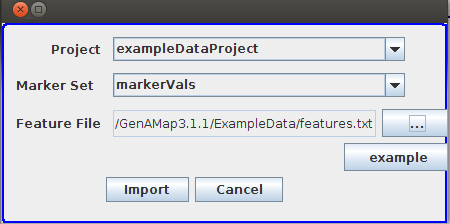
\includegraphics[width=\textwidth]{Figure7.png}
\caption{\textbf{Importing Feature Data}}
\label{features}
\end{figure}

\begin{figure}
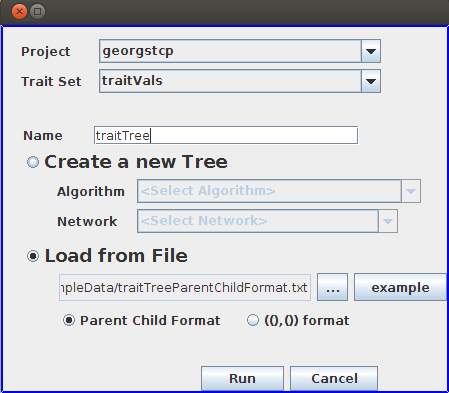
\includegraphics[width=\textwidth]{Figure8.png}
\caption{\textbf{Importing Tree Data}}
\label{tree}
\end{figure}

\begin{figure}
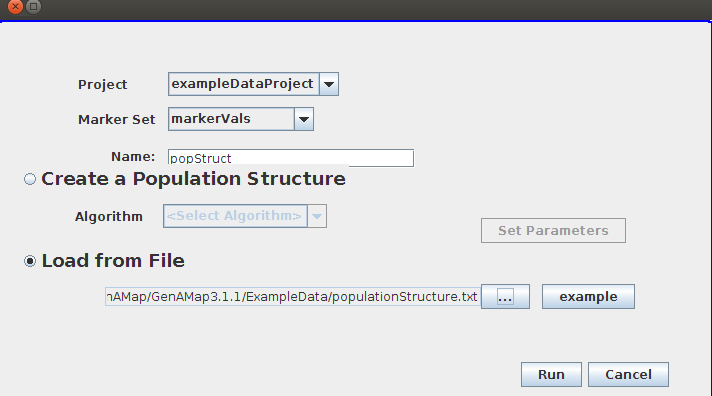
\includegraphics[width=\textwidth]{Figure9.png}
\caption{\textbf{Importing a Population Structure}}
\label{popstruct}
\end{figure}

\end{document}















